\documentclass{standalone}

\usepackage{tikz}
\usetikzlibrary{positioning}

% Paul Tol's qualitative palette ``bright''.https://personal.sron.nl/~pault/#sec:qualitative
\definecolor{tblue}{HTML}{4477AA}
\definecolor{tcyan}{HTML}{66CCEE}
\definecolor{tgreen}{HTML}{228833}
\definecolor{tyellow}{HTML}{CCBB44}
\definecolor{tred}{HTML}{EE6677}
\definecolor{tpurple}{HTML}{AA3377}
\definecolor{tgrey}{HTML}{BBBBBB}



\begin{document}

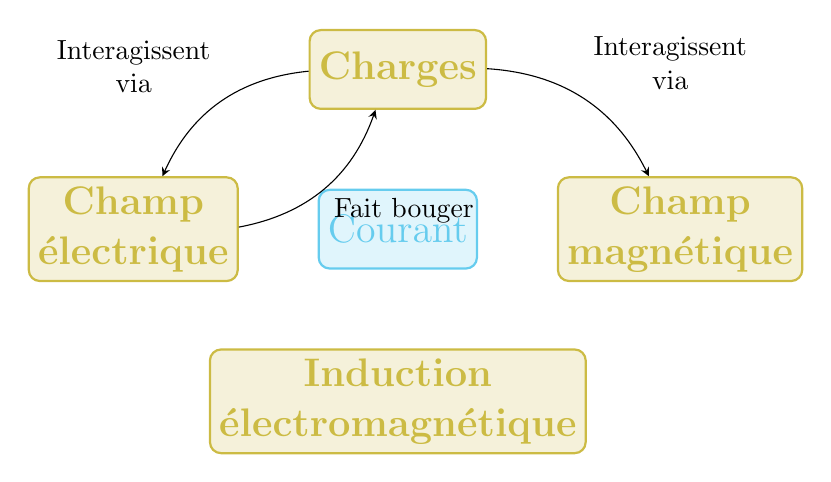
\begin{tikzpicture}[
    >=stealth,
    fondamental/.style={draw, rectangle, rounded corners, minimum height=1cm,
                        align=center, thick, tyellow, font=\Large\bfseries,
                        fill=tyellow, fill opacity=0.2, text opacity=1.0},
    secondaire/.style={draw, rectangle, rounded corners, minimum height=1cm,
                       align=center, thick, tcyan, font=\Large,
                       fill=tcyan, fill opacity=0.2, text opacity=1.0}
  ]
  \node[fondamental] (charge) {Charges};
  \node[secondaire] (courant) [below=of charge] {Courant};
  \node[fondamental] (E) [left=of courant] {Champ \\ électrique};
  \draw[->] (charge) to[bend right=30]  node[anchor=south east, align=center] {Interagissent \\ via} (E);
  \draw[->] (E) to[bend right=30]  node[anchor=north west, align=center] {Fait bouger} (charge);
  
  \node[fondamental] (B) [right=of courant] {Champ \\ magnétique};
  \node[fondamental] (L) [below=of courant] {Induction \\ électromagnétique};
  \draw[->] (charge) to[bend left=30]  node[anchor=south west, align=center] {Interagissent \\ via} (B);

  
\end{tikzpicture}

\end{document}